The microfluidic system made in this project is described in this section. It is defined as having an inlet and an outlet, where the liquid respectively enters and exits the device, fitted to soft Tygon thermoplastic tubing \cite{Olanrewaju2018}. The inlet tube is then linked to a glass syringe connected to a precise motor Syringe Pump by Cole-Parmer model CP-120 that compresses the syringe at a constant programmable rate. The SUT begins in the syringe, then flows in the tubes before entering the inlet. It then reaches the PDMS microchannel where it is sensed by the PCB electrodes linked to the Impedance Sensing Device. The liquid finally exits through the outlet tube, which is linked to a waste container. The PDMS channel and PCB electrodes are sealed tight by a system of 3d-printed squeezers that sandwich the channel and PCB electrodes together. Those are tightened together by screws, effectively sealing the microchannel and PCB electrode due to the flexible nature of PDMS. The microfluidic system is shown in \autoref{fig:MicrofluidicSystem} and illustrated in \autoref{fig:DiagramMicrofluidicSystem}. \par
\begin{figure}[h]
    \centering
    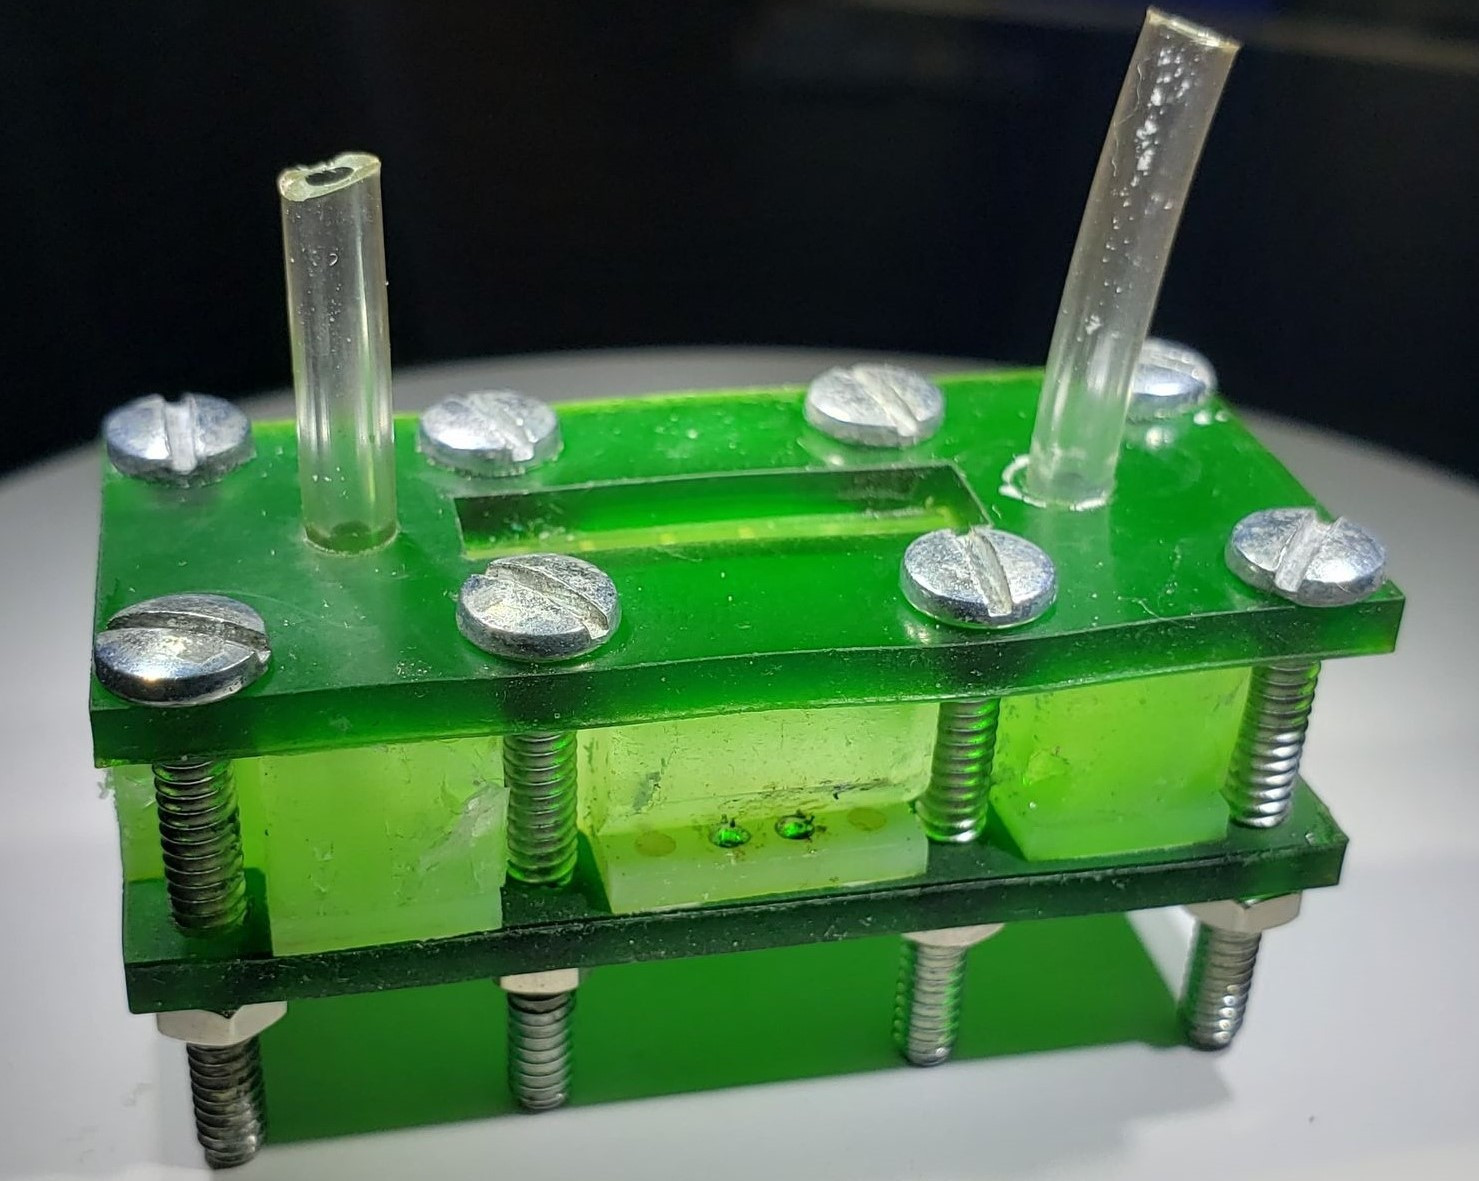
\includegraphics[width=0.6\textwidth]{MicrofluidicSystem}
    \caption{3d-printed microfluidic system used in this research to measure the impedance of a flowing liquid. It is composed of two 3d-printed squeezers, coplanar electrode pairs on PCB, a PDMS microchannel, soft tubes, and 8 screws and bolts.}
    \label{fig:MicrofluidicSystem}
\end{figure}
\begin{figure}[h]
    \centering
    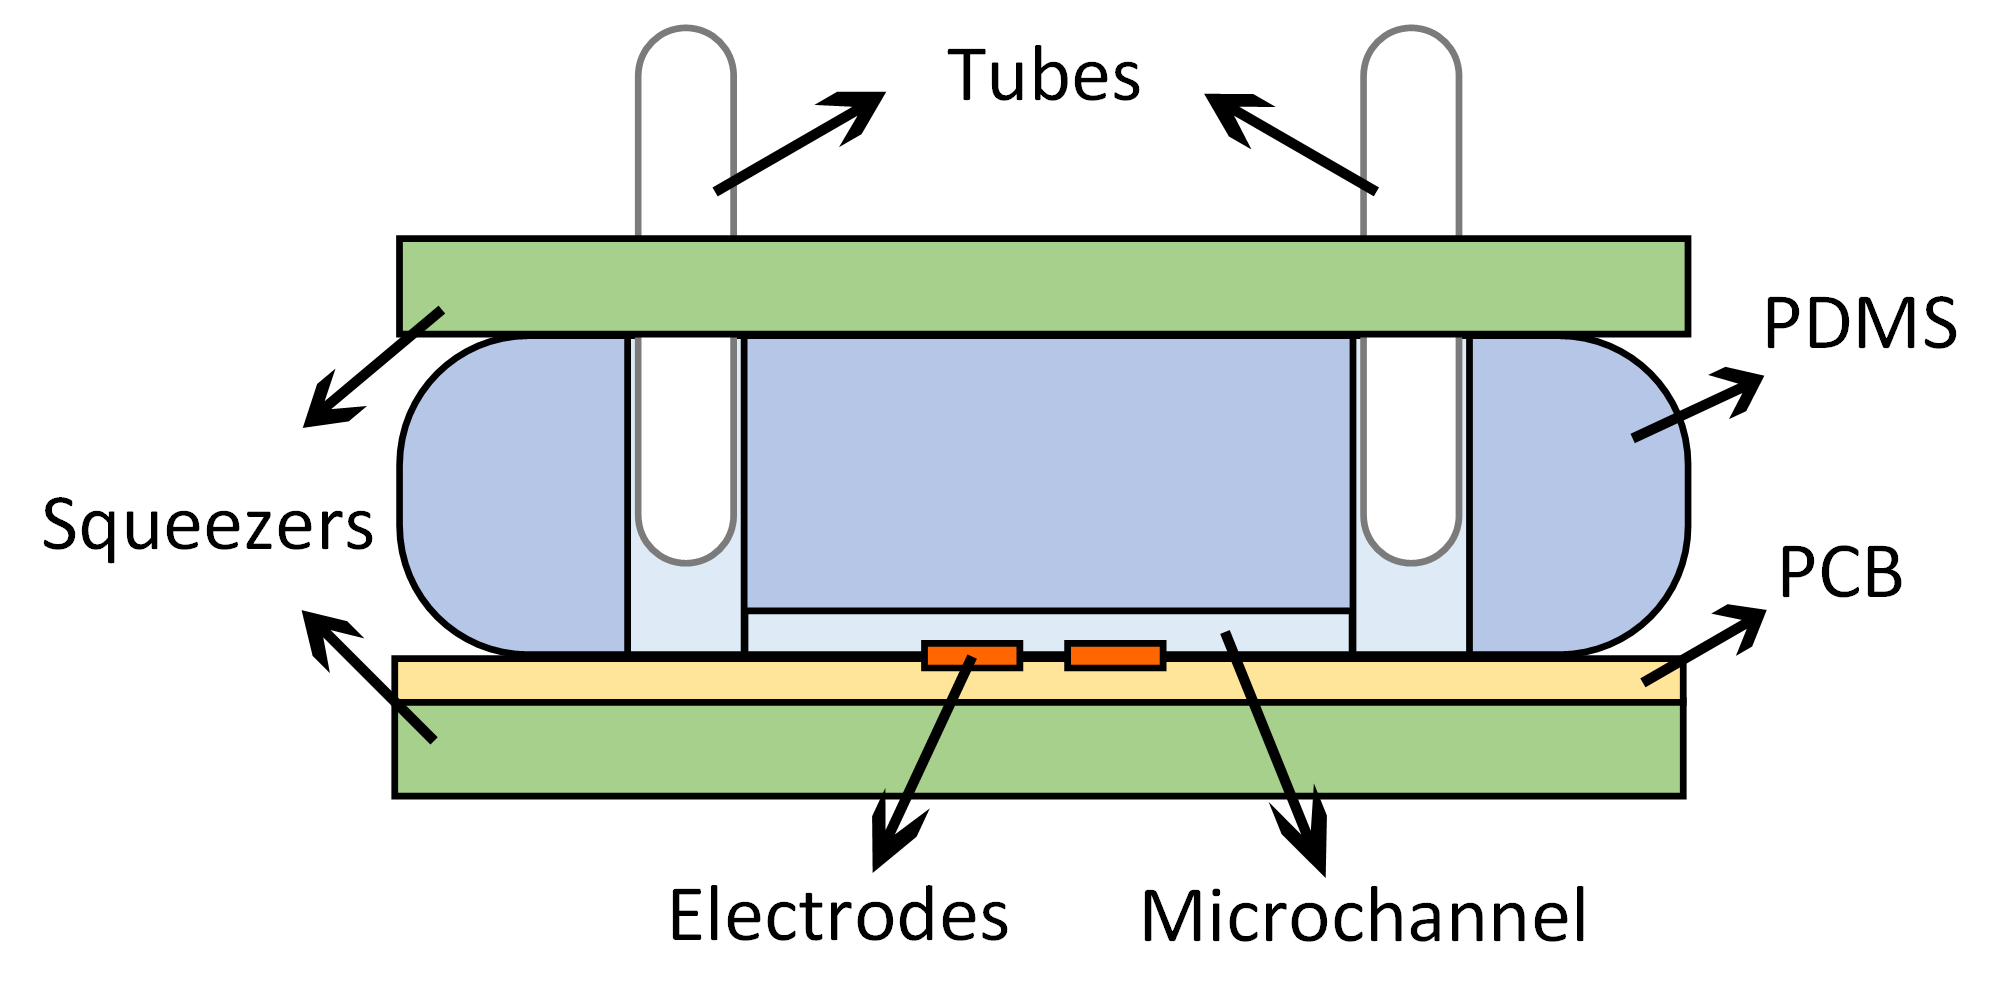
\includegraphics[width=0.9\textwidth]{DiagramMicrofluidicSystem}
    \caption{Diagram of the microfluidic system used in this research.}
    \label{fig:DiagramMicrofluidicSystem}
\end{figure}

The whole fabrication process is described in \autoref{fig:MicrofluidicsFabricationProcess}. A mold is initially realized on a CAD software such as Solidworks. This model is sent as a .STL file to the CADworks3D software to be meshed \cite{Cadworks3d}. This new meshed model is used in the software by the stereolithography 3d-printer CADworks3d H50-405 to print a 3d-mold using Master Mold for PDMS Device Photopolymer Resin \textsuperscript{TM} created by CADworks3D. The resin is then rinsed with IPA (90\%) or Methyl Hydrate for 5min and blow dried using an air gun. The mold is then cured using violet light in a LED light curing box machine (produced by Cadworks3d) sending wavelengths of 400nm for about 50min. PDMS (SYLGARD\textsuperscript{TM} 184 Silicone Elastomer Base) and a curing agent (SYLGARD\textsuperscript{TM} 184 Silicone Elastomer Curing Agent) are mixed at a ratio of 10:1 and degassed by letting the solution rest for 60min [48]. The mixture is put in the mold and cooked on a hot plate for 50min at 70° and dried overnight at 40° \cite{Trantidou2017}. A scalpel is used to gently prick-off the channel from the mold. The surfaces of the PDMS microchannel are exposed to plasma at 600 KPa for 1min. PEG is immediately put on the surface to keep its hydrophilicity for long periods of times. After waiting 10min, the PDMS microchannel is cooked 10min at 130° on a hot plate \cite{Trantidou2017}. A dry gun is blown on the channel to take away any residues. The PCB electrodes are aligned on the microchannel and a pressure is applied to seal them. Two 3d-printed squeezers are aligned at the top and bottom of the closed microchannel and screws are fitted to squeeze the PCB electrodes and PDMS microchannel in between the two squeezers. Finally, tubes are inserted at the inlet and outlet of the PDMS microchannel, concluding on the whole process. The microfluidic system is thus hermetic and easy to interact with. \par 
\begin{figure}[h]
    \centering
    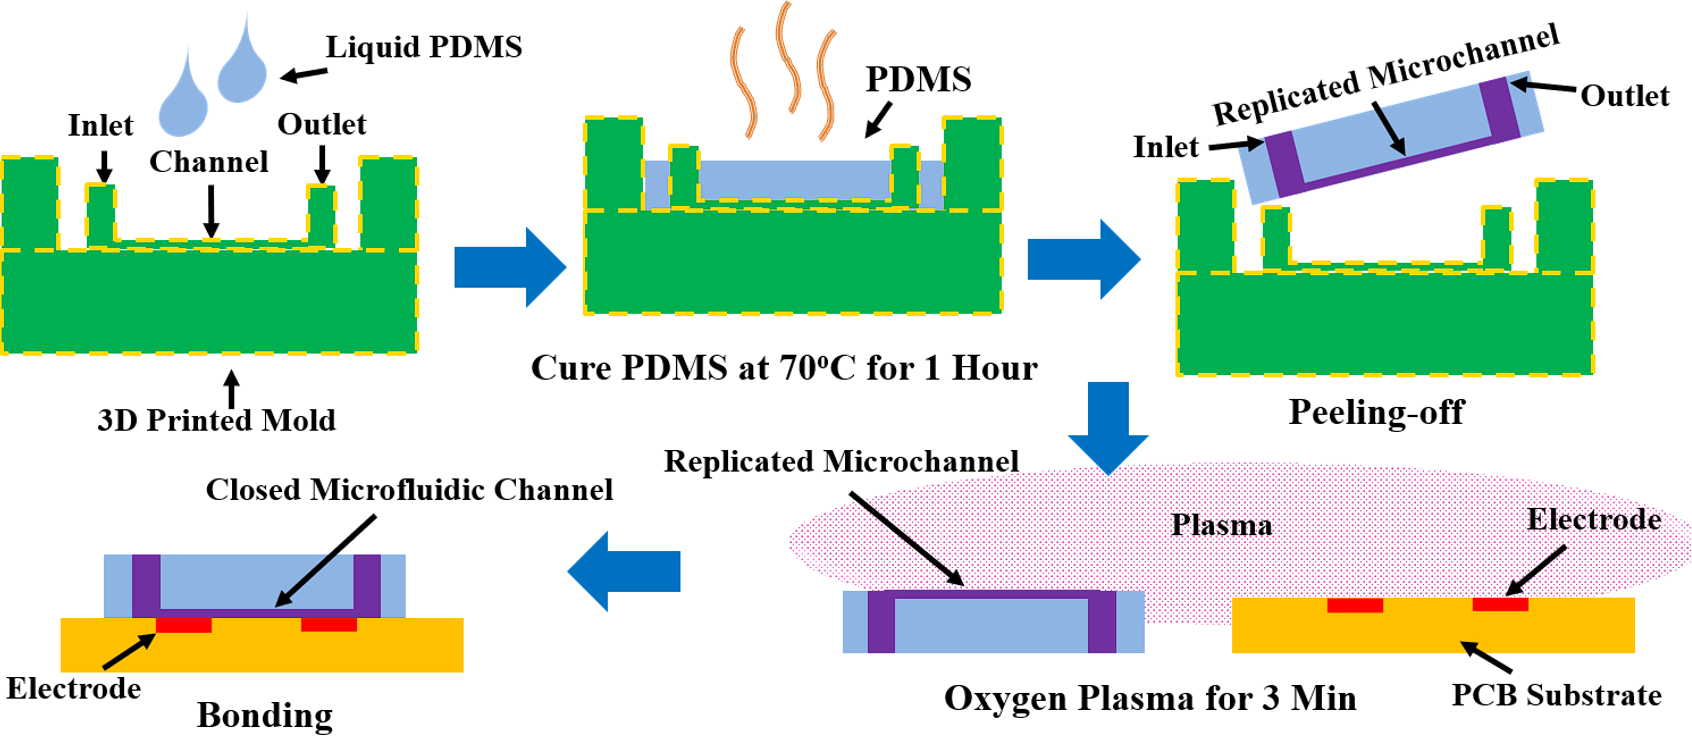
\includegraphics[width=0.99\textwidth]{MicrofluidicsFabricationProcess}
    \caption{Schematized steps for the fabrication process of the microfluidics system.}
    \label{fig:MicrofluidicsFabricationProcess}
\end{figure}

The shape of the mold is shown in \autoref{fig:3dprintedcomponents}. Using the H50-405, a theoretical resolution of 30 $\mu$m is possible, altough in practice, the minimum size of a channel possible to print without major defects is 90 $\mu$m. The PDMS cured in this mold solidifies into a structure with four openings in which the screws can be placed, as shown in \autoref{fig:PDMSChannel}. The electrode and squeezers share the same shape, as shown \autoref{fig:PCBElectrode2}.
%Scanning Electron Microscope (SEM) images were also taken to characterize the surface of the PDMS microchannel, as shown in \autoref{fig:SEMPDMS}
\begin{figure}[h]
\centering
%\begin{subfigure}{0.99\textwidth}
%\centering
    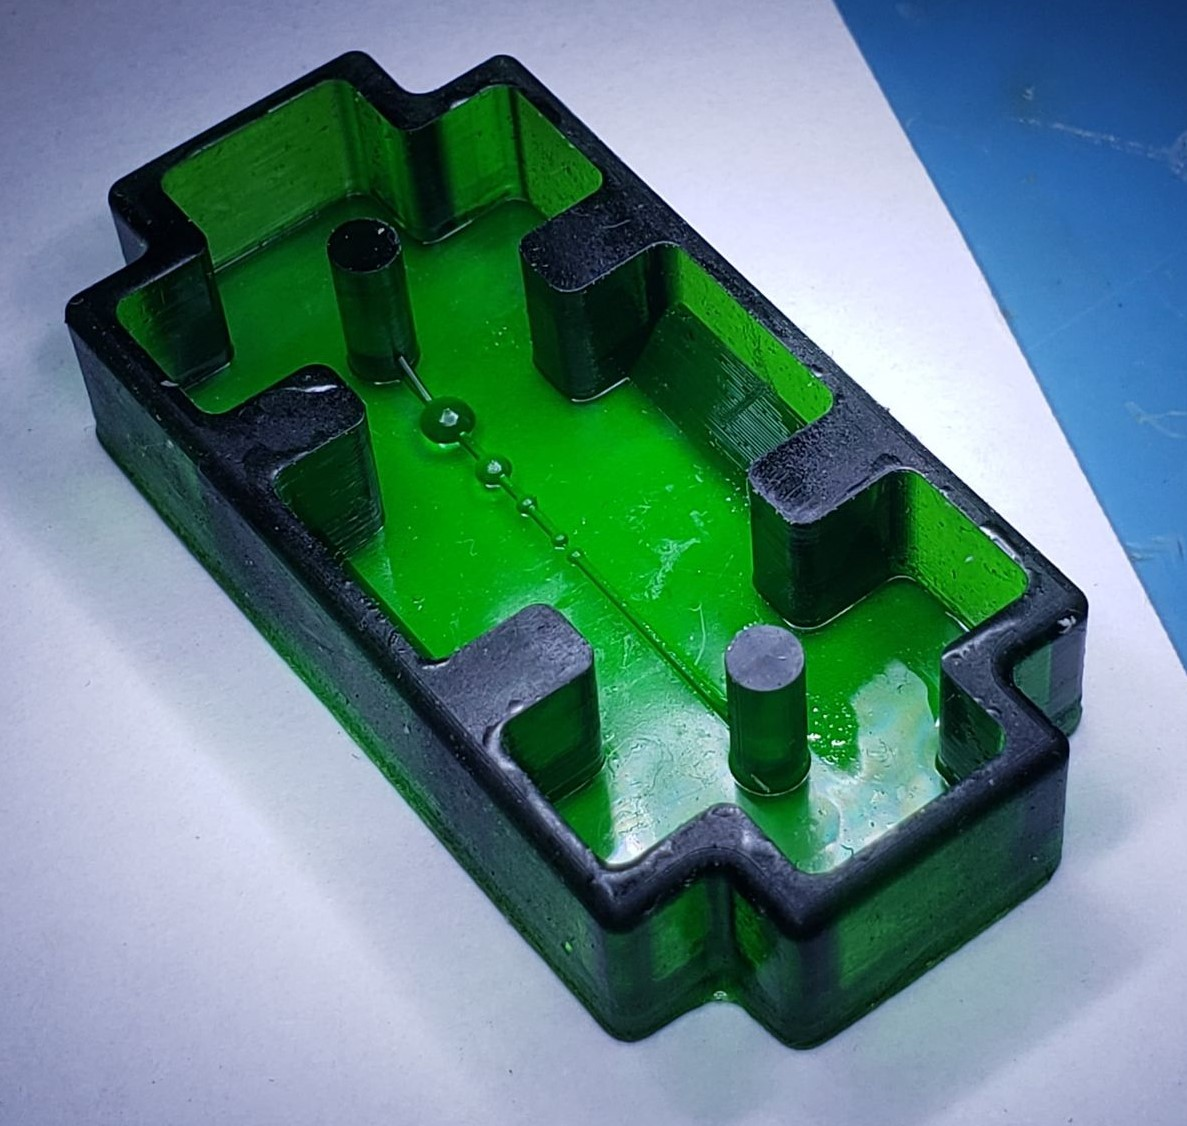
\includegraphics[width=0.8\linewidth]{Mold}
    %\caption{Mold.}
    %\label{fig:Mold}
%\end{subfigure}
%\begin{subfigure}{0.49\textwidth}
%\centering
%    \includegraphics[width=0.99\linewidth]{Squeezers}
%    \caption{Squeezers.}
%    \label{fig:Squeezers}
%\end{subfigure}
\caption{3d-printed mold of the microfluidic system.}
\label{fig:3dprintedcomponents}
\end{figure}

\begin{figure}[h]
\centering
\begin{subfigure}{0.49\textwidth}
\centering
    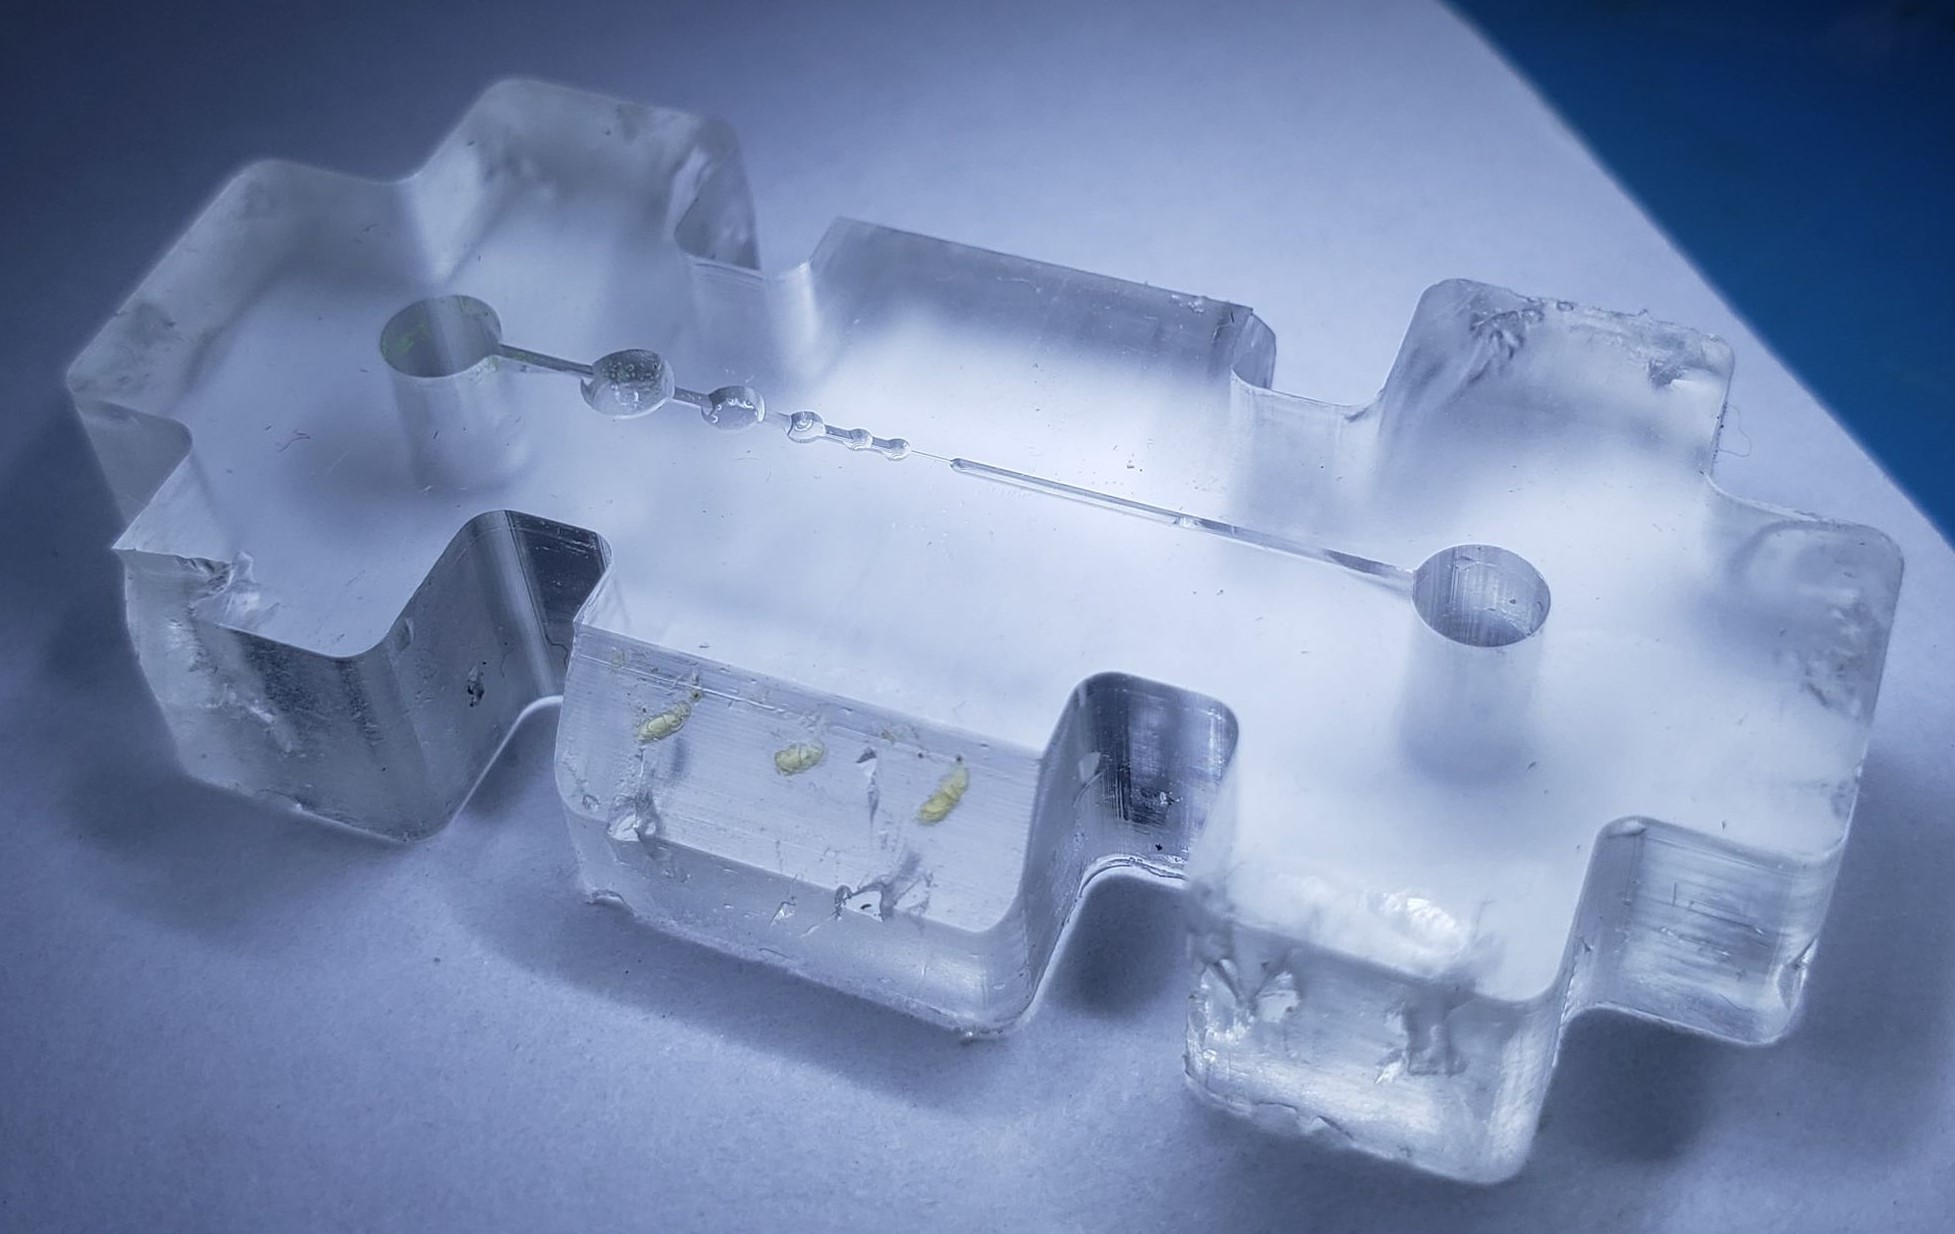
\includegraphics[width=0.88\linewidth]{FullChannel}
    \caption{Full view.}
    \label{fig:FullChannel}
\end{subfigure}
\begin{subfigure}{0.49\textwidth}
\centering
    \includegraphics[width=0.99\linewidth]{ZoomedChannel}
    \caption{Zoomed view.}
    \label{fig:ZoomedChannel}
\end{subfigure}
\caption{Solidified PDMS microchannel cured in the 3d-printed mold.}
\label{fig:PDMSChannel}
\end{figure}

%\begin{figure}[h]
%    \centering
%    \includegraphics[width=0.7\textwidth]{SEMPDMS}
%    \caption{SEM images of the surface of the PDMS microchannel. }
%    \label{fig:SEMPDMS}
%\end{figure}

The electrodes are fabricated on a one-layer PCB and were fabricated by PCBWay. They have a size of 46 $\times$ 21 $\times$ 1.6 mm. They are constructed from the conventional substrate FR-4 TG130 with smaller spacings of 4mils in the exact shape of the microfluidic channel so that they both might be fitted on top of one another. Finally, the surface finish is immersion gold (ENIG) (1U") with 1oz copper. These electrodes are 101.6 $\mu m$ wide and are separated by 101.6$\mu m$. Refer to \autoref{sec:ElectrodeDesign} for additional information on electrode-design. \par
\begin{figure}[h]
\centering
\begin{subfigure}{0.49\textwidth}
\centering
    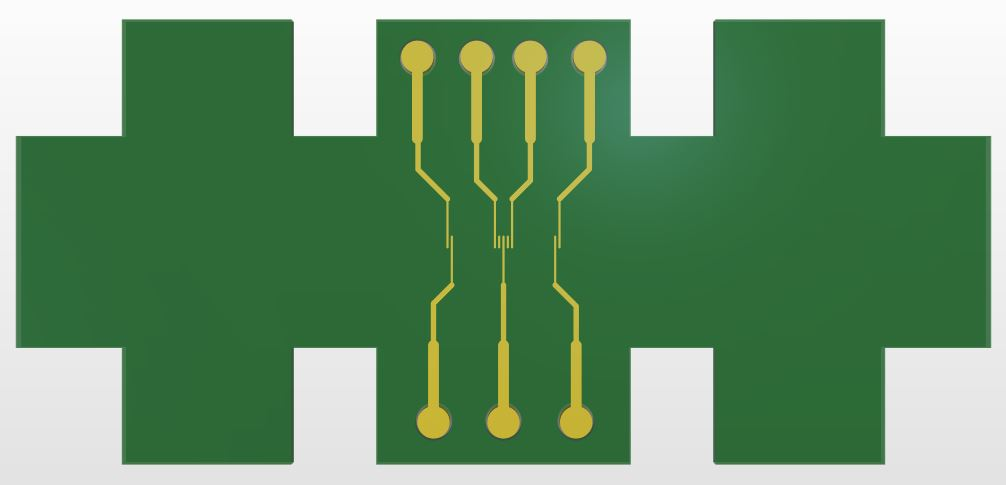
\includegraphics[width=0.99\linewidth]{PCBElectrode2}
    \caption{Full view.}
    \label{fig:PCBElectrode2}
\end{subfigure}
\begin{subfigure}{0.49\textwidth}
\centering
    
\includegraphics[width=0.7\linewidth]{PCBElectrode1}
    \caption{Zoomed view.}
    \label{fig:PCBElectrode1}
\end{subfigure}
\caption{3d-model of the electrodes on PCB as represented in Altium Designer.}
\label{fig:AltiumPCBElectrode}
\end{figure}

The 5-electrode configuration described in \citep{De_Ninno2017} has been chosen for this study. It creates a pattern in the observed signal that can be used to estimate the position of the cell in the channel. This is obtained at the price of a reduction in sensibility since the electrodes are further spaced apart from one another when arranged such. The 3d-model of the PCB electrode model, as represented in Altium Designer, is shown in \autoref{fig:AltiumPCBElectrode}, and the actual PCB electrodes are shown in \autoref{fig:PCBElectrode}. The aligment between the microchannel and electrodes is shown in \autoref{fig:AlignedElectrode}.

\begin{figure}[h]
\centering
\begin{subfigure}{0.49\textwidth}
\centering
    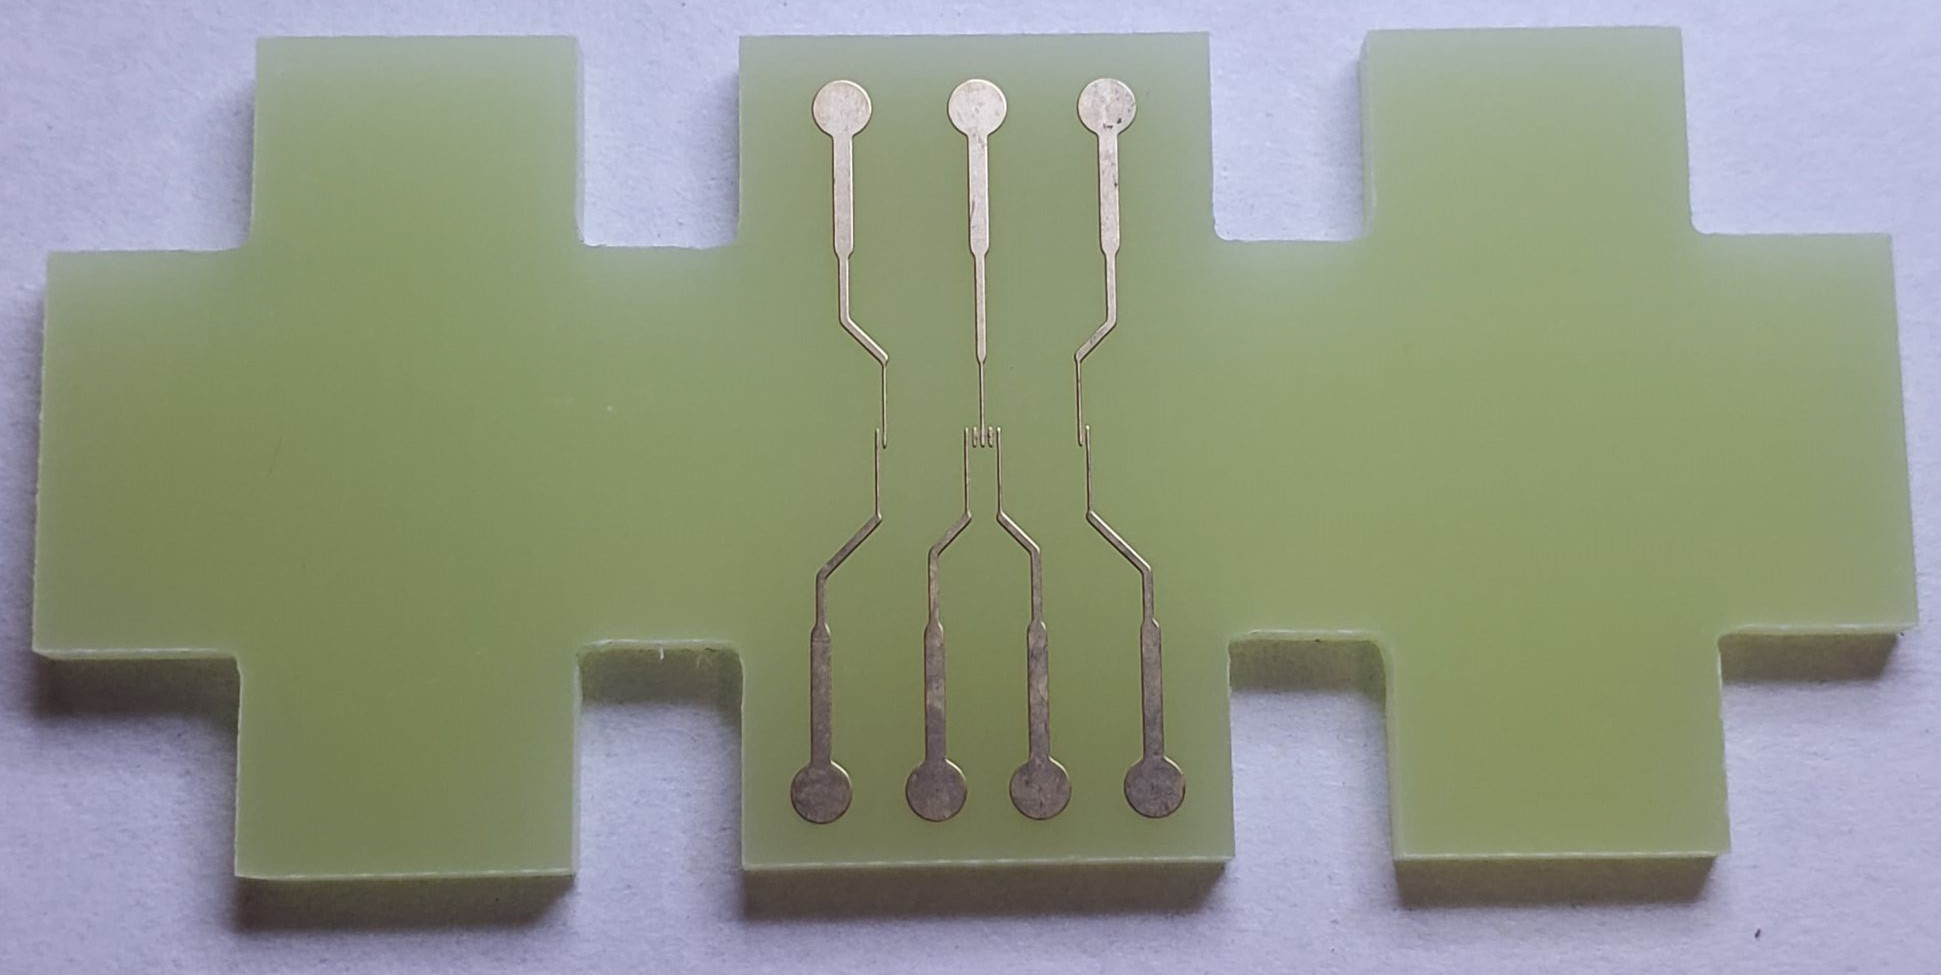
\includegraphics[width=0.96\linewidth]{PCBElectrode3}
    \caption{Full view.}
    \label{fig:PCBElectrode3}
\end{subfigure}
\begin{subfigure}{0.49\textwidth}
\centering
    \includegraphics[width=0.9\linewidth]{PCBElectrode4}
    \caption{Zoomed view.}
    \label{fig:PCBElectrode4}
\end{subfigure}
\caption{Practical electrodes on PCB.}
\label{fig:PCBElectrode}
\end{figure}

\begin{figure}[h]
    \centering
    \includegraphics[width=0.99\textwidth]{AlignedElectrode}
    \caption{PDMS microchannel alligned with the electrodes. }
    \label{fig:AlignedElectrode}
\end{figure}